% Chapter Template

\chapter{Graphene-SGX} % Main chapter title

\label{Chapter3} % Change X to a consecutive number; for referencing this chapter elsewhere, use \ref{ChapterX}

\section{Introduction}
Intel SGX技术提供了一系列的硬件特性,帮助保护应用免受操作系统、hypervisor、BIOS和其他软件的伤害。
应用程序可以整个或者部分的放入到enclave中运行,而enclave会有如下功能
\begin{itemize}
    \item 对enclave内的虚拟地址空间的机密性和完整性进行保护。
    \item 限制控制流进入enclave的入口。
    \item 启动时检查内存的内容。
    \item 远程证明。
\end{itemize}

正是因为提供了这些功能,因此用户就可以放心的将他们的敏感应用或者敏感数据放在云服务提供商的enclave中去运行,保证
自己敏感应用的安全性,大大增加了云服务能够服务的对象。
\paragraph{SGX的适配较为困难}为了保证SGX的安全性,在SGX中运行的应用将有一些限制。
比如应用不能在enclave中调用syscall,而是通过一层shielding code去访问syscall,通过sheld层,syscall的结果
在返回给应用之前会被验证,保证结果的安全可靠,防止host的操作系统攻击enclave中的应用。因此,普遍认为
应用程序适配SGX需要付出大量的努力。
前人的工作 Haven \cite{186173}展示了可以利用一个 library OS 把没有修改过的应用放到SGX中去。
但是这需要付出性能上的 overhead 和TCB的扩大的代价。
不过,Graphene-SGX验证了实际上利用library OS带来的overhead并没有前人所称的那么大,
利用Graphene-SGX可以快速的把现有的应用放到enclave中去运行,并且没有很大的开销。

\paragraph{Graphene-SGX并不是最优的}
Graphene-SGX这一工作的目的并不是为了追求更好的SGX技术利用性能,
而是为了把已有工作更快的部署到enclave中去。
因此,虽然有很多方法可以提升enclave代码中的性能,
降低代码的TCB,
但是enclave都暂未采用,因为这些优化会令应用的适配更加复杂。



\section{威胁模型}
Graphene-SGX 的威胁模型与典型的 SGX 应用的威胁模型类似。
下列的组件是不被信任的:
\begin{itemize}
    \item [1)] 
    除CPU之外的硬件。
    \item [2)]
    操作系统、hypervisor和其他的系统软件。
    \item [3)]
    在enclave之外跟其他enclave之内运行的应用程序。
    \item [4)]
    同一应用程序的enclave之外的部分。
\end{itemize}   
\paragraph{}
Graphene-SGX只信任CPU,还有enclave内部的代码(shielding module、bootloader)。
还必须信任Intel的SGX SDK中的aesmd工具,该工具验证enclave签名中的属性并批准enclave的创建。
这是现在利用SGX技术的所有工作都必须信任的。
除此之外,虽然Graphene-SGX使用且仅使用了Intel SGX SDK 中的驱动程序,但是并不信任他。

\section{保证的安全性质和能够防御的一些具体攻击}
\subsection{保证的安全性质}
\paragraph{继承自SGX的性质}
Graphene-SGX 是对SGX技术的应用,因此,Intel SGX 技术提供的保护也被完全的继承。
1)对enclave内的虚拟地址空间的机密性和完整性进行保护。
2)限制控制流进入enclave的入口。
3)启动时检查内存的内容。
4)连接Intel服务器进行远程证明

\paragraph{Graphene-SGX提供的特性}
除此之外,Graphene-SGX还提供了很多其他安全性质。
例如:
\begin{itemize}
    \item 通过本地验证证明两个本地enclave是安全的。
    \item 在两个安全的本地enclave之间搭建安全通信。
    \item 提供安全的fork机制创建一个新的enclave。
\end{itemize}

\subsection{能够防御的具体攻击}
\begin{itemize}
    \item [1)]\textbf{来自host上其他进程的攻击} memory corruption,ROP attack
    \item [2)]\textbf{自host OS 的攻击}rootkits
    \item [3)]\textbf{来自硬件的攻击}cold-boot attacks
\end{itemize}

\section{性能、可扩展性(scalability)、灵活性等分析}
\subsection{灵活性和可扩展性}
由于Graphene-SGX可以直接在enclave上运行没有经过修改的Linux程序,因此,通过Graphene-SGX可以快速的
帮助现有应用利用到SGX的enclave这一特性,提高已有应用的安全性,而同时不需要付出太大的开发成本。

在可扩展性方面,Graphene-SGX还提供了enclave的fork操作,用户可以简单的通过一个enclave环境,
fork出一个新的子enclave环境。
同时 Graphene-SGX 还提供了两个enclave之间的加密通信,互相验证的功能。
因此,多进程的应用程序可以有效的保留多进程抽象的同时利用SGX技术带来的安全保证。


\subsection{性能分析}
\begin{figure}[]
    \centering
    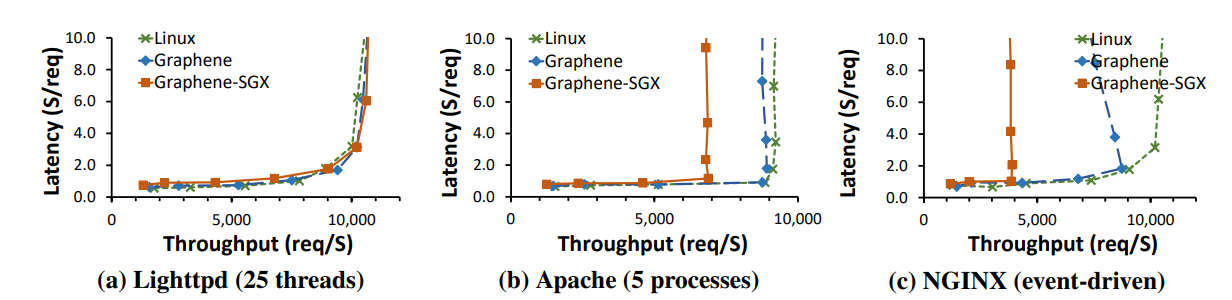
\includegraphics[width=1\textwidth]{1.png}    
    \caption{三种应用(Lighttpd、Apache、NGINX)
    分别在Linux、Graphene、Graphene-SGX环境下的性能表现}
    \label{23333}
\end{figure}
图\ref{23333}展示了Graphene-SGX的性能分析。
可以从途中看出,对轻量级的网站服务应用\textbf{Lighttpd}来说,
Graphene-SGX对性能的影响不大。对\textbf{Apache}来说,由于Apache服务器有多个worker,
每个worker在一个enclave环境中,因此worker之间的通信,请求的传输,
都需要用到enclave之间的加密通信,会消耗很大的性能。
因此,如果不用SGX的话,单独的Graphenen技术并不会带来多少的overhead,但是如果要保证安全性,
对性能就会产生影响。
\textbf{NGINZ}服务器由事件驱动,因此Graphene的shielding 层对数据的检查会有overhead,因此性能更差。

不过,由于Graphene-SGX主要致力于将应用快速的部署到SGX提供的enclave中去,所以很多性能优化的工作都未集成。
在已有快速部署已有应用这一特性的前提下,Graphene-SGX的性能对先前工作来说也是很有竞争力的。


\section{不足}
\paragraph{无法防御一些攻击}
Denial of service,sidechannels,controlled-channel attacks这些攻击是目前所有的 SGX 平台都难以防御的,Graphene-SGX同样无法处理。
\paragraph{不能保证可用性}
像其他的利用SGX的平台一样,
Graphene-SGX可以保证代码在enclave内部的安全执行,
但是无法保证enclave本身的可用性。
例如,恶意的操作系统可以一直不返回到enclave中,或者在某些需要等待的操作中提前返回enclave使受保护的代码执行超出预期。



%----------------------------------------------------------------------------------------
%	SECTION 1
%----------------------------------------------------------------------------------------
